\documentclass{article}


\usepackage{arxiv}

\usepackage[utf8]{inputenc} % allow utf-8 input
\usepackage[T1]{fontenc}    % use 8-bit T1 fonts
\usepackage{hyperref}       % hyperlinks
\usepackage{url}            % simple URL typesetting
\usepackage{booktabs}       % professional-quality tables
\usepackage{amsfonts}       % blackboard math symbols
\usepackage{enumitem}
% \usepackage{nicefrac}       % compact symbols for 1/2, etc.
% \usepackage{microtype}      % microtypography
% \usepackage{lipsum}
\usepackage{graphicx}
% \voffset=-0.5in
% \voffset=0.5in
% \hoffset=-0.5in

\title{Motion-Based Handwriting Recognition }

% \vspace{-30pt}
\author{
  Junshen Kevin Chen \\
  Stanford University\\
  \texttt{jkc1@stanford.edu} \\
  %% examples of more authors
   \And
  Wanze Xie \\
  Stanford University\\
  \texttt{wanzexie@stanford.edu} \\
    \And
  Yutong He \\
  Stanford University\\
  \texttt{kellyyhe@stanford.edu} \\
}

\begin{document}
% \vspace{-30pt}
\maketitle

% \begin{abstract}
% This is the milestone report for our final project. In the work so far, we have formalized data collection methodology and collected a small sample of preliminary data. This report also discusses some of the key strategies in organizing and processing data for our training work. Then, a preliminary K-means and a K-Medoids model is introduced as a baseline. Finally, this report discusses some of the potential future plans.
% \end{abstract}


% ============================== begin content ==============================
\vspace{-15pt}
\section{Motivation}

It is prevalent in today’s world for people to write on a touch screen with a smart pen, as there is a strong need to digitize hand-written content, to make the review and indexing easier. However, despite the success of character recognition on digital devices \cite{bib1} \cite{bib2} \cite{bib3}, requiring a digitizer as the writing surface poses a possibly unnecessary restriction to be overcome. In addition, in VR and AR applications, it is also hard to recognize the texts written with the motion sensors \cite{bib4} \cite{bib5}.

We propose a solution by using a pen equipped with motion sensor to predict the words written by the user. Instead of using image data or on-screen stroke data, we analyze the acceleration and gyroscopic data of the pen using machine learning techniques to predict the characters and words the user is writing. 


\section{Data Collection}

Since the project proposal, we have made improvements to the hardware and established a formalized data collection strategy. Figure \ref{fig:hardware} in Appendix \ref{hardware_appendix} shows the finalized data collection hardware built using Arduino and the recording button (left), and the handwriting guide grid with pen (right).

In a data collection session, we perform the following:
\begin{enumerate}[topsep=0pt,itemsep=-1ex,partopsep=1ex,parsep=1ex]
    \item Record stationary frame data of roughly 10 seconds, this data is then averaged and used to calibrate the sensor in data processing time.
    \item Inform the subject to write each lowercase letter in the English alphabet 20 times, each time in a separate box drawn on the board; when writing each letter, the subject would: (1) move pen to starting position; (2) press button; (3) write; (4) stop writing; (5) release button.
\end{enumerate}

We define each event of writing one English letter, starting when button pressed and ending when released as a \textbf{writing event}, the sequence of data that belongs to one writing event as a \textbf{data sequence}, and a sample that belongs to a particular data sequence as a \textbf{data sample}.

We have collected data from 3 subjects among ourselves. Appendix \ref{data_format} shows the detailed format and an example of our collected data. We have also implemented a data augmentation pipeline, described in Appendix \ref{data_augmentation} due to the difficult nature of our data collection process.




\section{Data Exploratory Analysis}

\subsection{Data Interpolation and Re-sampling}

For some models that do not have the inherent structure for time series data, such as CNN, right after performing calibration and normalization as in Appendix \ref{calibration}, we want to flatten the data sequence to a 1-D vector. However, there are two problems in doing this directly: (1) subjects write in different speed, and therefore some writing of the same letter may produce a longer sequence than others and hence produce vectors with different length; (2) the sensor samples in a variable rate, and therefore the time delta between each timestamp varies.

To solve these problems, we design a procedure that normalizes data sequences so that they have the same the number of features. For the desired number of features $3 \times N$, where $N$ is the average number of data samples in each data sequence for all letters, do:

\begin{enumerate}
    \item Extract the yaw, pitch, roll values separately from each data sequence and create a $3\times1$ array for them;
    \item Map the yaw, pitch, roll values to corresponding accumulated timestamps;
    \item Create a 1D linear interpolation model for each data sequence;
    \item Generate linearly spaced time stamps based on the lower and upper bound of the original timestamps;
    \item Calculate the interpolated yaw, pitch, roll value for each timestamp generated in step 4;
    \item Pair up corresponding yaw, pitch, roll values and merge them into a single vector of length $3 \times N$;
\end{enumerate}

% We run this re-sampling process for every data sequence and a demonstration of the output will be like the following:

% \begin{center}
%     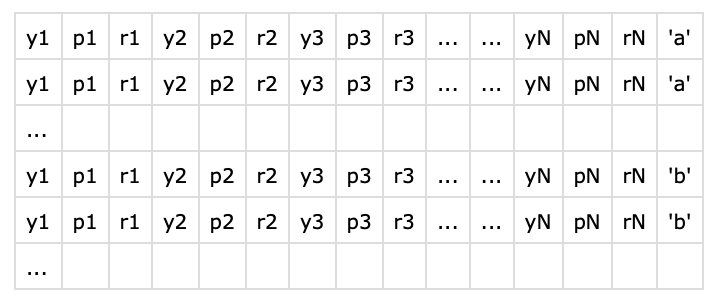
\includegraphics[scale=0.5]{flatten.png}
% \end{center}

\subsection{Data Visualization}

\begin{center}
    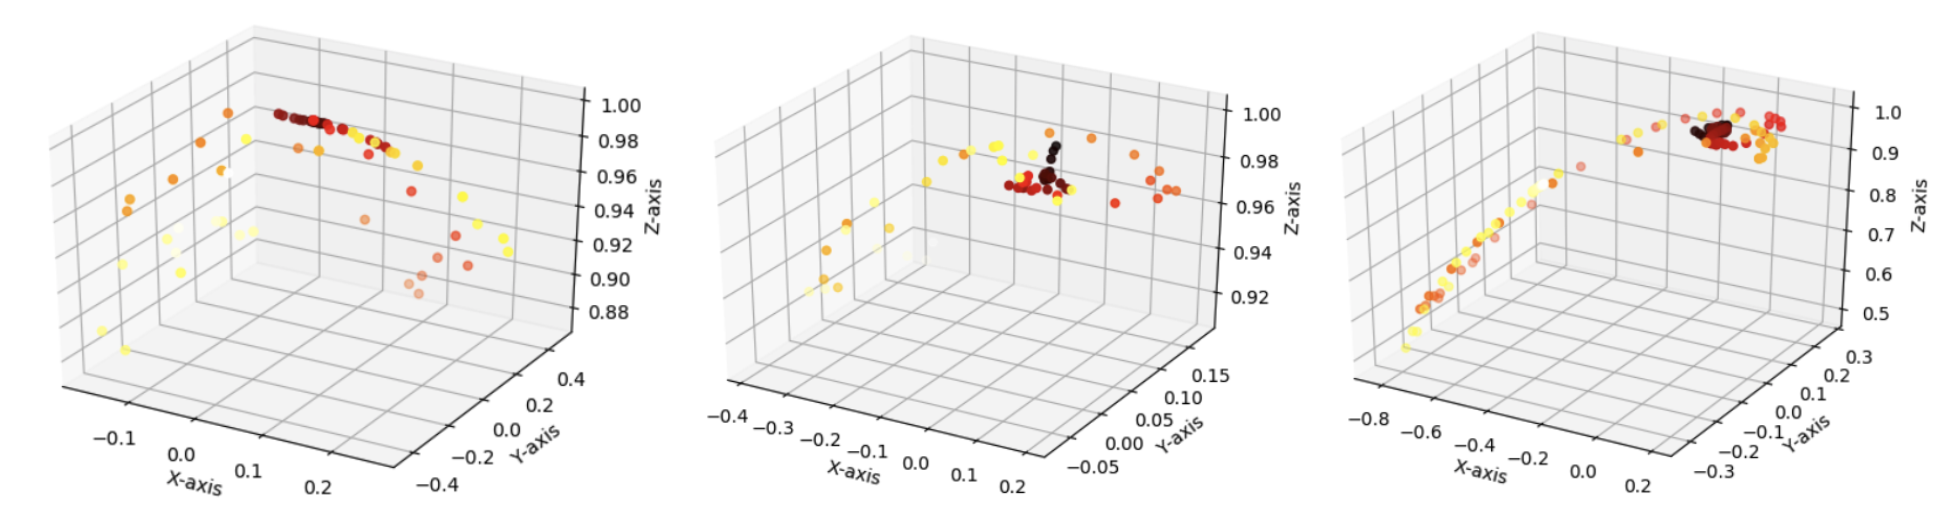
\includegraphics[scale=0.2]{a-3-subject.png}
    
    \textit{Traces of lowercase 'a' written by 3 subjects.}
\end{center}

\begin{center}
    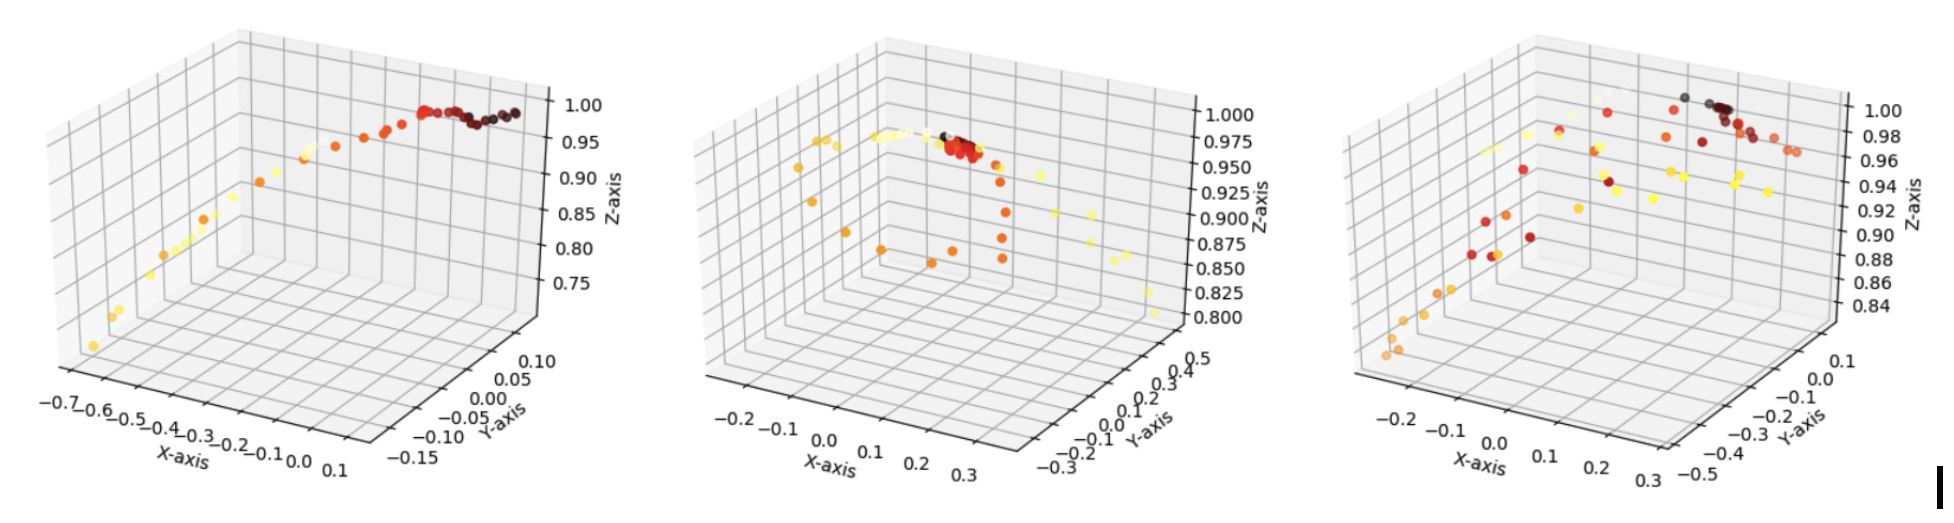
\includegraphics[scale=0.2]{loy.png}
    
    \textit{Traces of lowercase 'l', 'o', 'y' written by the same subject.}
\end{center}

The above visualization is achieved by using the rotation sensor values to rotate a unit vector, then placing the vector from the origin, and plotting the other end of the vector in a 3D space. The colors from dark to light indicates the accumulated time stamps from the beginning.

Observing the above, even though the traces of rotation values do not resemble the letter itself, mainly due to the sensor records the tail of the stylus, we notice that writing of the same letter share characteristics across subjects, and distinct letters have identifiable traces against each other.


\section{Baseline Model: K-means and K-Medoids for Classification}

\subsection{Methods and Motivation}

We choose to experiment with K-Means and K-Medoids because of the similarity nature in human's writing. I.e., there are shared ways for people to write English alphabets. As a result, algorithms that can group similar data can be ideal for this problem. We do not chose KNN classification method due to its inefficiency at prediction/test time.

We first implement K-means and K-Medoids algorithm for $k$ in the range of 26 to 51, to tackle the letter recognition problem. K-means and K-Medoids are both unsupervised learning algorithms, in which the samples are randomly initialized to be assigned to $K$ clusters, then iterate until convergence. The implicit objective function minimizes the distances of sample to its assigned cluster:

\[
J(x,c,z) = \sum_{i=1}^n \sum_{j=1}^K \mathbf{1}\{z^{(i)} = j\} \|x^{(i)} - c_j\|^2
\]

In the future, we plan to also incorporate distance functions such as Dynamic Time Warping\cite{bib8} that are more meaningful to the time series data. After convergence, the model assigns a label to each cluster as the most popular label of the samples in the cluster. For prediction, the model finds the closest cluster centroid to the new sample and yield the label of the cluster.

\subsection{Preliminary Results and Analysis}

\begin{table}[ht]
\centering
\begin{tabular}{|l | c c c |}
\hline
Methods       & Best K & Training Accuracy & Test Accuracy   \\ \hline \hline
K-Means       & 48     & 0.4807692         & 0.1615385      \\ 
K-Medoids     & 44     & 0.4576923         & 0.1807692      \\ \hline
% K-Medoids DTW & 20     &                   & 0.12153846      \\ \hline
\end{tabular}
\centering
\end{table}

We use data from two subjects for training and the other one for testing. The above result shows that the K-Means and K-Medoids algorithms cannot achieve very optimal results both in training and testing settings, although they both achieved non-trivial predictions of each testing data as the accuracy is above which from random guess ($0.0385$). Table \ref{results} Appendix \ref{result_appendix} also shows that, as the number of clusters increases, training and testing accuracy have the tendency to increase as well. This suggests that our choice of baseline models suffer from the problem of high bias, since when we increase the number of parameters, it benefits both the training and testing accuracy. On the other hand, because of the limited amount of data, this model also has very high variance, since there is a large gap between the training and testing accuracy.

We also observe that both algorithms do not achieve their best accuracy at $k = 26$. We attribute this to the fact that some characters have more than one way to be written. Some drawbacks of building a K-means/K-Medoids model and making predictions by considering the closest cluster is that it is stroke-order sensitive and data-inefficient: because the input to the K-means/K-Medoids model is a normalized and flattened array of frames in the sequence, this clustering is not invariant to different stroke orders or writing speed. For example, if subject A writes the letter "f" in a different order than another subject B, then the K-means/K-Medoids cluster produced with subject A's data would not be able to generalize to subject B. As a result, to obtain a well generalized model, we need to collect from a large number of subjects with different writing habits.


\section{Next Steps}

\subsection{Data Collection}

We plan to collect data from 17 more subjects, producing a final data set of 20 subjects. In the meantime, we also plan to incorporate the currently unused attributes of information to augment the performance of our models.

\subsection{Neural Network}

Using interpolation and re-sampling techniques, we are able to reshape data points such that the sequence from each writing event is of the same dimension. We can flatten this data to a vector and use it to train an 1 dimensional \textbf{Convolutional Neural Network (CNN)} for classification. The input will have $N$ features with $3$ channels. 

The objective function to minimize for a multi-class classification problem is Cross Entropy:

\[
J(x, y) = - \sum_{i=1}^n \sum_{c=1}^C y_c^{(i)} \log \hat{y}_c^{(i)}
\]

Since each writing sequence is unique in length. Then, without using interpolation to force each sample to be the same length, we can use the time series to train a \textbf{Recurrent Neural Network (RNN)} such as Long Short-Term Memory (LSTM) \cite{bib7} to perform the same classification task. The loss function to optimize is same as the above.

\subsection{Evaluation}

Finally, we will evaluate the performance across different models trained to see and analyze which performs better than the others. We will also convert the same data set into (albeit noisy) 2-D images and train an OCR model, and compare the performance to our motion-based models.

\section*{Contribution}

All team members contributed to the overall building of this project, collecting data , and writing this report.
\textbf{Kevin} built a pipeline for data collection and calibration, data loading, pre-processing, preliminary visualization.
\textbf{Wanze} built the hardware, implemented the interface for collecting data from hardware, designed methods for processing raw motion data, and created functions for re-sampling and interpolation.
\textbf{Yutong} implemented data augmentation pipeline, and designed and conducted the preliminary experiments.


\bibliographystyle{unsrt}  

\begin{thebibliography}{1}
    \bibitem{bib1} Maximilian Schrapel, Max-Ludwig Stadler, and Michael Rohs. 2018. Pentelligence: Combining Pen Tip Motion and Writing Sounds for Handwritten Digit Recognition. In Proceedings of the 2018 CHI Conference on Human Factors in Computing Systems (CHI '18). ACM, New York, NY, USA, Paper 131, 11 pages. DOI: https://doi.org/10.1145/3173574.3173705
    \bibitem{bib2} Jacob O. Wobbrock, Brad A. Myers, and John A. Kembel. 2003. EdgeWrite: a stylus-based text entry method designed for high accuracy and stability of motion. In Proceedings of the 16th annual ACM symposium on User interface software and technology (UIST '03). ACM, New York, NY, USA, 61-70. DOI: https://doi.org/10.1145/964696.964703 
    \bibitem{bib3} “US6839464B2 - Multiple Pen Stroke Character Set and Handwriting Recognition System with Immediate Response.” Google Patents, Google, https://patents.google.com/patent/US6839464B2/en.
    \bibitem{bib4}  I. Poupyrev, N. Tomokazu, and S. Weghorst. 1998. Virtual Notepad: Handwriting in Immersive VR. In Proceedings of the Virtual Reality Annual International Symposium (VRAIS '98). IEEE Computer Society, Washington, DC, USA, 126-.
    \bibitem{bib5} “US10067568B2 - Augmented reality writing system and method thereof.” Google Patents, Google, https://patents.google.com/patent/US10067568B2/en
    \bibitem{bib6} Hamed Habibi Aghdam and Elnaz Jahani Heravi. 2017. Guide to Convolutional Neural Networks: A Practical Application to Traffic-Sign Detection and Classification (1st ed.). Springer Publishing Company, Incorporated.
    \bibitem{bib7} Sepp Hochreiter and Jürgen Schmidhuber. 1997. Long Short-Term Memory. Neural Comput. 9, 8 (November 1997), 1735-1780. DOI=http://dx.doi.org/10.1162/neco.1997.9.8.1735
    \bibitem{bib8} Stan Salvador and Philip Chan. 2007. Toward accurate dynamic time warping in linear time and space. Intell. Data Anal. 11, 5 (October 2007), 561-580.
\end{thebibliography}

\appendix
\section*{Appendix}
\section{Data Collection Hardware} \label{hardware_appendix}
\begin{figure}[ht]
    \centering
    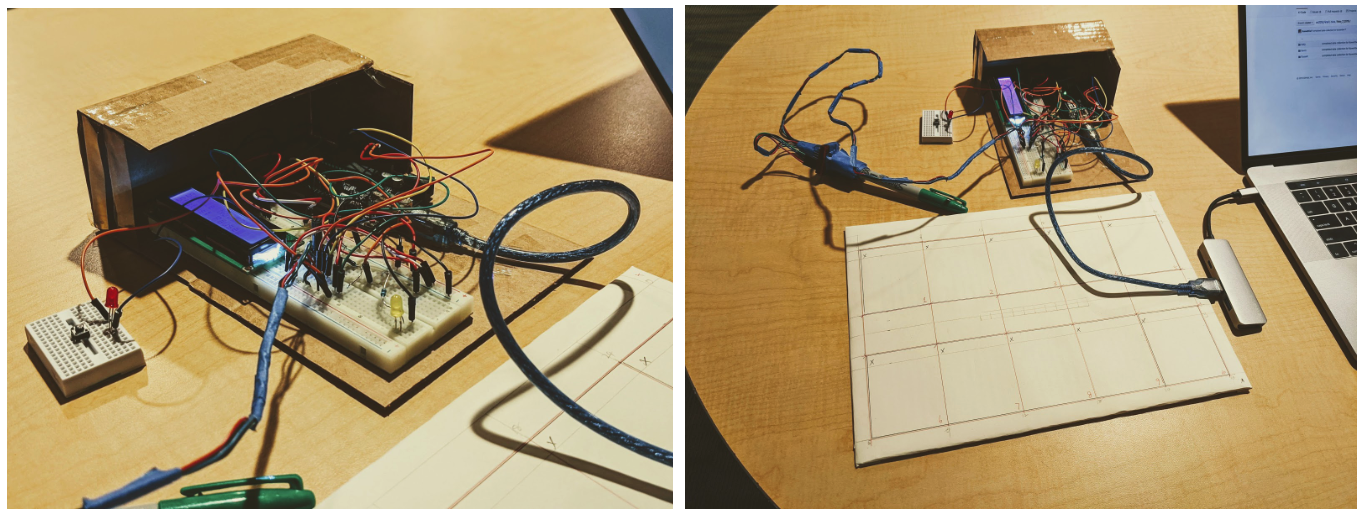
\includegraphics[scale=0.25]{hardware.png}
    \caption{The hardware we built for data collection.}
    \label{fig:hardware}
\end{figure}

% \begin{figure}[h!]
%     \centering
%     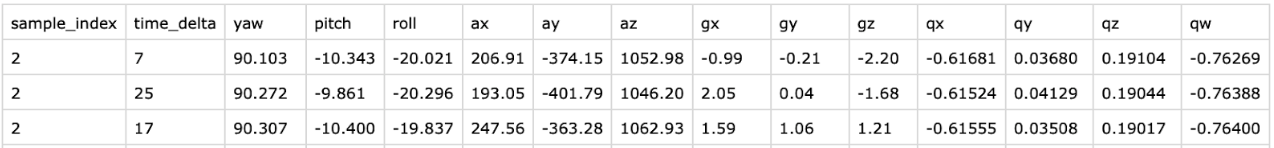
\includegraphics[scale=0.35]{data-table-sample.png}
%     \caption{Sample data}
%     \label{fig:hardware2}
% \end{figure}


\section{Data Format} \label{data_format}

Each letter written by each subject is then uniquely identified by the subject name and the label $\{a, ..., z\}$ .

Each sequence is stored as one row in csv format, where there are the following columns:

\begin{enumerate}
    \item \texttt{sample\_index}: the data that belongs to the same writing event / sequence has the same sample\_index
    \item \texttt{time\_delta}: the time difference between the current data and previous data (in \small{$milliseconds$})
    \item \texttt{yaw, pitch, roll}: rotation values around each axis (in \small{$degrees$})
    \item \texttt{ax, ay, az}: acceleration on each axis (in \small{$mm/s^2$})
    \item \texttt{gx, gy, gz}: gyroscopic velocity on each axis (in \small{$degrees/s$})
    \item \texttt{qx, qy, qz, qw}: quaternion representation of the absolute rotation 
\end{enumerate}

\begin{figure}[ht]
    \centering
    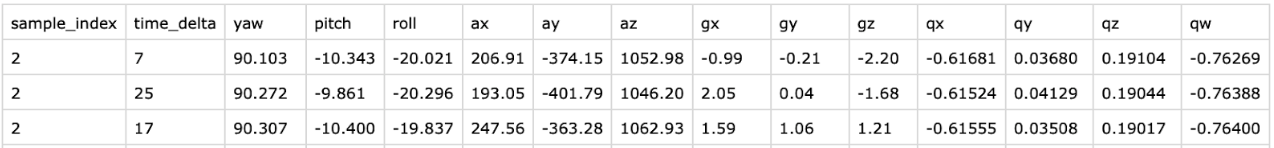
\includegraphics[scale=0.35]{data-table-sample.png}
    \caption{An example of the collected data.}
    \label{fig:data_example}
\end{figure}

% \begin{table}[ht]
% \centering
% \begin{tabular}{|l | c c c |}
% \hline
% Methods       & Best K & Training Accuracy & Test Accuracy   \\ \hline \hline
% K-Means       & 48     & 0.4807692         & 0.1615385      \\ 
% K-Medoids     & 44     & 0.4576923         & 0.1807692      \\ \hline
% % K-Medoids DTW & 20     &                   & 0.12153846      \\ \hline
% \end{tabular}
% \centering
% \end{table}


\section{Calibration and Normalization} \label{calibration}

To correct calibration error, we take the mean of the calibration recording and subtract it to all frames in all samples.

For some columns, such as yaw, pitch, roll, we want the training data to be invariant to the absolute rotation of the pen (i.e. some subject might be holding the pen differently, but writing the letter in the same way). We get around the issue by subtracting frame 0 from all frames.


\section{Data Augmentation} \label{data_augmentation}

Due to the high difficulty of collecting a large amount of data, we implemented a data augmentation pipeline to rotate, stretch and add noise to each written letter collected. For each data point collected, we first convert it into a matrix with each column containing the yaw, pitch, roll information respectively, and each row representing the data of a certain time stamp.

Given an input matrix, we are able to 

\begin{enumerate}[nolistsep]
    \item Add a Gaussian noise centered at 0 and with customized variance to each entry;
    \item Rotate the object counter-clockwisely by a quaternion vector;
    \item Stretch each row by three scalar constants corresponding to yaw, pitch, roll
\end{enumerate}

\section{Preliminary Experiment Comprehensive Results} \label{result_appendix}
The table displays on the next page.
\begin{table}[ht]
\centering
\begin{tabular}{|c|c|c|c|c|}
\hline
\textbf{K}&\textbf{KMeans Train}&\textbf{KMeans Test}&\textbf{KMedoids Train}&\textbf{KMedoids Test} \\ \hline \hline
26 & 0.2711538462 & 0.06538461538 & 0.3038461538   & 0.09807692308 \\ 
27 & 0.3038461538 & 0.1192307692  & 0.3173076923   & 0.1269230769  \\ 
28 & 0.3134615385 & 0.09230769231 & 0.3826923077   & 0.1019230769  \\ 
29 & 0.2884615385 & 0.1134615385  & 0.3173076923   & 0.1096153846  \\ 
30 & 0.3403846154 & 0.09423076923 & 0.2865384615   & 0.1192307692  \\ 
31 & 0.325        & 0.09230769231 & 0.2942307692   & 0.08269230769 \\ 
32 & 0.2942307692 & 0.1038461538  & 0.3692307692   & 0.1730769231  \\ 
33 & 0.3807692308 & 0.1211538462  & 0.3384615385   & 0.1307692308  \\ 
34 & 0.3576923077 & 0.1           & 0.3211538462   & 0.1615384615  \\ 
35 & 0.3692307692 & 0.08076923077 & 0.3269230769   & 0.1076923077  \\ 
36 & 0.3538461538 & 0.1057692308  & 0.3134615385   & 0.1076923077  \\ 
37 & 0.3653846154 & 0.08269230769 & 0.3519230769   & 0.1269230769  \\ 
38 & 0.3769230769 & 0.1076923077  & 0.3423076923   & 0.1173076923  \\ 
39 & 0.3788461538 & 0.07307692308 & 0.3480769231   & 0.1615384615  \\ 
40 & 0.3519230769 & 0.1019230769  & 0.3192307692   & 0.1076923077  \\ 
41 & 0.3769230769 & 0.09615384615 & 0.3653846154   & 0.1230769231  \\ 
42 & 0.4057692308 & 0.1326923077  & 0.3423076923   & 0.08846153846 \\ 
43 & 0.375        & 0.1615384615  & 0.4211538462   & 0.08846153846 \\ 
44 & 0.4057692308 & 0.1192307692  & 0.4576923077   & 0.1807692308  \\ 
45 & 0.3596153846 & 0.09038461538 & 0.4269230769   & 0.1826923077  \\ 
46 & 0.3692307692 & 0.08653846154 & 0.4057692308   & 0.1634615385  \\ 
47 & 0.4519230769 & 0.1403846154  & 0.3634615385   & 0.1076923077  \\ 
48 & 0.4807692308 & 0.1153846154  & 0.4384615385   & 0.1826923077  \\ 
49 & 0.4057692308 & 0.1384615385  & 0.4019230769   & 0.1692307692  \\ 
50 & 0.3865384615 & 0.1096153846  & 0.4115384615   & 0.1038461538  \\ 
51 & 0.4403846154 & 0.07884615385 & 0.3884615385   & 0.1230769231  \\ \hline
\end{tabular}
\centering
\vspace{10pt}
\caption{The complete results of our preliminary experiment.}
\label{results}
\end{table}


% \begin{table}[ht]
% \centering
% \begin{tabular}{|l | c c c |}
% \hline
% Methods       & Best K & Training Accuracy & Test Accuracy   \\ \hline \hline
% K-Means       & 48     & 0.4807692         & 0.1615385      \\ 
% K-Medoids     & 44     & 0.4576923         & 0.1807692      \\ \hline
% % K-Medoids DTW & 20     &                   & 0.12153846      \\ \hline
% \end{tabular}
% \centering
% \end{table}

\end{document}


